\documentclass{article}
\usepackage{graphicx}
\usepackage[margin=1in]{geometry}
\usepackage[outdir=./]{epstopdf}  					% Avoids errors when input figures
\usepackage[labelsep=period,labelfont=bf]{caption}
%\usepackage{subcaption}

\begin{document}
\begin{figure}[tbph]
\caption{Long-Horizon Forecasts of Inflation} \label{fig:wnCPI}
\begin{center}								% center the minipage on the line
	\begin{minipage}{0.9\linewidth}
	\begin{center}							% center the figure inside the minipage
	\includegraphics[trim={0cm 0cm 0cm 0cm},clip,height=0.82\textheight,width=\linewidth]{../Figures/Surveys/wnCPI.eps} \\
	\end{center}
	\fignotes{This figure plots the 5-years ahead (dashed line) and the 5- to 10-years ahead or long-term (solid line) average consumer price inflation forecasts against the survey date. For Israel and South Africa, the figure shows the inflation trend, see appendix \ref{sec:trendinf}. The figure also includes the upper and lower bounds for the domestic inflation target, where applicable. The upper and lower bounds are the most recent ones for each country. For Russia, since it has updated its target range almost every year since early 2000s, the plotted band shows the highest and lowest bounds since 2009.}
	\end{minipage}
\end{center}
\end{figure}
\end{document}
% trim = {<left> <lower> <right> <upper>}